% Capítulo 5: Desarrollo del proyecto
\section{Introducción}
\label{sec:des-intro}

El capítulo anterior expuso el diseño del sistema: su arquitectura en el modelo C4, su descomposición funcional y de casos de uso, su comportamiento dinámico, y los marcos de calidad (sección~\ref{sec:prop-calidad}) y de seguridad (sección~\ref{sec:prop-seguridad}) que orientan la construcción. Este capítulo presenta la materialización de ese diseño en un prototipo funcional: el código fuente que lo implementa y su organización en el repositorio, las pantallas del prototipo en operación, y el análisis de seguridad de la implementación, que contrasta los controles previstos en el diseño con los efectivamente construidos.

\section{Código fuente del proyecto}
\label{sec:des-codigo}

El código fuente completo del sistema se encuentra publicado en un repositorio de GitHub, lo que permite su revisión, su reproducción y el seguimiento de su historial de desarrollo:

\begin{center}
\url{https://github.com/antoniotorresxd/ia-spice}
\end{center}

El repositorio se organiza como un monorepositorio con tres aplicaciones independientes bajo el directorio \texttt{project/apps/}, en correspondencia directa con los contenedores del nivel 2 del modelo C4 (sección~\ref{subsec:prop-c4-nivel2}):

\begin{itemize}
    \item \texttt{client/} — el subsistema cliente: una aplicación web construida con React y TypeScript sobre Vite, que concentra la autenticación, los espacios de trabajo y la interfaz desde la que el usuario envía sus solicitudes en lenguaje natural.
    \item \texttt{server/} — la API del sistema: un servicio construido con el framework Hono sobre el runtime Bun, con Better Auth para la autenticación, Drizzle ORM sobre PostgreSQL (Neon) para la persistencia, y validación de esquemas con Zod. Expone, además de las rutas de autenticación, el catálogo de configuraciones de LLM que consume el subsistema de agentes.
    \item \texttt{agents/} — el ecosistema de agentes: un proyecto en Python 3.12 que implementa, sobre LangGraph, el grafo de orquestación descrito en el capítulo anterior —orquestador, cálculo (Master-Worker), síntesis (escritura y shell) y curador— con PySpice para la generación de netlists y el motor ngspice para la simulación.
\end{itemize}

Cada aplicación gestiona sus propias dependencias con su gestor correspondiente (\texttt{npm}, \texttt{bun} y \texttt{uv}, respectivamente) y cuenta con su propia suite de pruebas automatizadas, cuyos resultados se documentan en el capítulo de pruebas. El historial de \textit{commits} del repositorio registra la evolución incremental del desarrollo, con mensajes bajo la convención \textit{conventional commits} que distinguen funcionalidades, correcciones, pruebas y documentación.

\section{Pantallas del prototipo funcional}
\label{sec:des-pantallas}

Las siguientes capturas muestran el prototipo funcional en operación y evidencian que el subsistema cliente materializa los casos de uso de acceso y de solicitud de generación descritos en la sección~\ref{subsec:prop-casos-uso}.

La pantalla de inicio de sesión (figura~\ref{fig:pantalla-login}) es la puerta de entrada al sistema. En su panel derecho ofrece el formulario de autenticación por correo y contraseña —delegada en Better Auth, conforme al diseño de seguridad— junto con las opciones de registro de cuenta nueva. El panel izquierdo comunica la propuesta del sistema y presenta la \textit{ruta de solución}: el diagrama de estados del pipeline de generación (entrada, orquestador, cálculo, síntesis, curador y los estados terminales de aceptación y rechazo), de modo que el usuario conoce, desde el acceso, el proceso de validación iterativa que seguirá su solicitud.

\begin{figure}[H]
    \centering
    \makebox[\textwidth][c]{%
        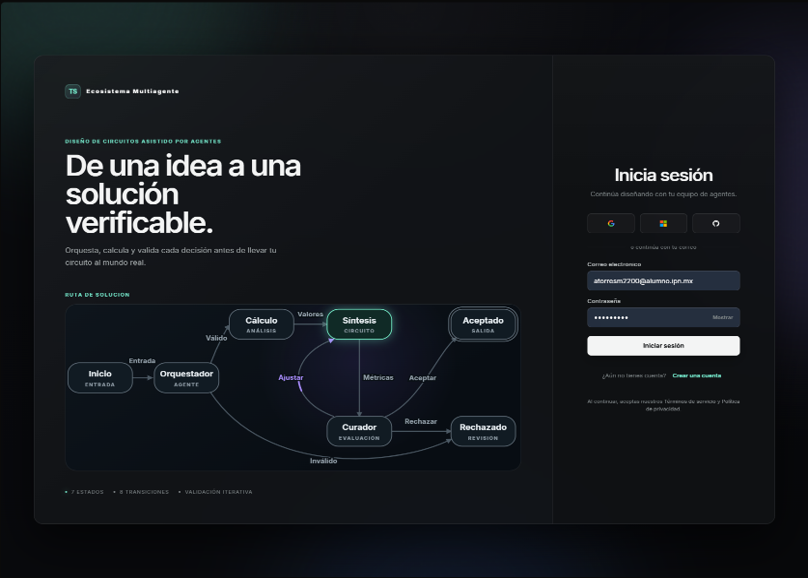
\includegraphics[width=1\textwidth, keepaspectratio]{../src/pantallas/Picture1.png}%
    }
    \caption{Pantalla de inicio de sesión del prototipo, con la ruta de solución del pipeline de generación.}
    \label{fig:pantalla-login}
\end{figure}

Tras autenticarse, el usuario accede a su espacio de trabajo personal (figura~\ref{fig:pantalla-workspace}). La pantalla de inicio concentra el caso de uso central del sistema: el campo de solicitud en lenguaje natural (``Describe qué quieres diseñar''), desde el cual se envía la descripción del circuito que desencadena el flujo de generación. La pantalla ofrece además un resumen operativo del consumo del periodo —tokens utilizados, costo estimado, tasa de solicitudes exitosas y tiempo procesado—, la actividad reciente con el estado de cada solicitud (completada, en proceso o que requiere atención), los proyectos que agrupan las conversaciones del usuario, y los archivos producidos por las generaciones (netlists \texttt{.cir}, resultados \texttt{.csv} y esquemáticos \texttt{.svg}). El asistente conversacional, visible en la esquina inferior, acompaña la interpretación de resultados y el ajuste de restricciones.

\begin{figure}[H]
    \centering
    \makebox[\textwidth][c]{%
        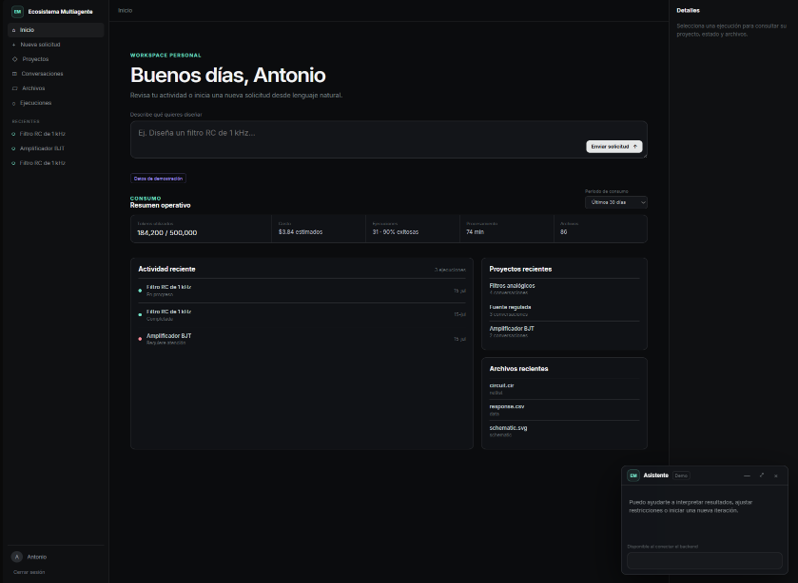
\includegraphics[width=1\textwidth, keepaspectratio]{../src/pantallas/Picture2.png}%
    }
    \caption{Espacio de trabajo autenticado: solicitud en lenguaje natural, resumen operativo, actividad reciente y archivos generados.}
    \label{fig:pantalla-workspace}
\end{figure}

\section{Análisis de seguridad de la implementación}
\label{sec:des-seguridad}

El marco de seguridad de la sección~\ref{sec:prop-seguridad} estableció los activos del sistema, los principios que ordenan su protección —confidencialidad, integridad y disponibilidad— y los controles previstos en el diseño. Esta sección analiza la implementación construida: verifica qué controles quedaron efectivamente implementados, con qué mecanismos concretos, y qué riesgos residuales permanecen. El análisis se realizó mediante revisión del código fuente del repositorio, contrastando cada control del diseño con el módulo que lo implementa.

\subsection{Controles implementados}
\label{subsec:des-seg-controles}

\textbf{Autenticación y gestión de sesiones.} La autenticación se delega en Better Auth, montada en el servidor bajo la ruta \texttt{/api/auth}. Las sesiones se gestionan mediante cookies configuradas según el entorno: en producción se emiten con el atributo \texttt{Secure} —que restringe su transmisión a HTTPS— y la política \texttt{SameSite} adecuada al despliegue de cliente y servidor en orígenes distintos; en desarrollo se emplea \texttt{SameSite=Lax}. Un middleware de sesión resuelve el usuario en cada solicitud, y las rutas protegidas anteponen una guarda (\texttt{requireAuth}) que responde 401 ante solicitudes no autenticadas, de modo que la autorización se aplica por ruta y no queda a criterio de cada handler.

\textbf{Cifrado de secretos en reposo.} Las API keys de los proveedores de LLM que el administrador registra en el catálogo se cifran antes de persistirse en la base de datos con AES-256-GCM, un esquema de cifrado autenticado que protege tanto la confidencialidad como la integridad del dato: una clave alterada en la base de datos no se descifra silenciosamente, sino que falla la verificación de autenticidad. La clave de cifrado (\texttt{LLM\_SECRETS\_KEY}) reside únicamente en una variable de entorno. Las vistas públicas del catálogo nunca devuelven la clave descifrada; la API key solo se descifra para entregarse al subsistema de agentes por el canal interno autenticado.

\textbf{Autenticación entre servicios.} La comunicación entre el subsistema de agentes y el servidor —necesaria para que el orquestador obtenga la configuración activa del LLM— se realiza mediante un endpoint interno protegido por un token de servicio (\texttt{AGENTS\_SERVICE\_TOKEN}) transmitido como credencial \textit{Bearer}. La verificación del token emplea comparación en tiempo constante (\texttt{timingSafeEqual}), lo que neutraliza los ataques de temporización que podrían inferir el token midiendo diferencias en el tiempo de respuesta. El subsistema de agentes no almacena la clave del LLM en disco: la conserva en una caché en memoria de vida corta (60 segundos), lo que acota la ventana de exposición.

\textbf{Validación de configuración y manejo de secretos.} El servidor valida la totalidad de sus variables de entorno con un esquema de Zod al arrancar y termina el proceso si la configuración es inválida o incompleta, lo que impide que el sistema opere en un estado degradado —por ejemplo, sin clave de cifrado o con un token de servicio débil (el esquema exige una longitud mínima)—. Ningún secreto se encuentra escrito en el código ni versionado en el repositorio: los archivos \texttt{.env} quedan fuera del control de versiones, en cumplimiento del requisito de manejo de secretos (RIMP-11).

\textbf{Control de orígenes cruzados.} El servidor aplica una política CORS con lista explícita de orígenes permitidos, leída de configuración, con soporte de credenciales. Esto impide que páginas de orígenes arbitrarios realicen solicitudes autenticadas contra la API aprovechando la sesión del usuario.

\textbf{Contención de la entrada en lenguaje natural.} La descripción del usuario no fluye libremente por el sistema: el orquestador exige al LLM una salida estructurada que se valida contra el esquema Pydantic de la especificación de circuito, y toda especificación —provenga del LLM o del camino estructurado— pasa por la misma validación y normalización antes de entrar al pipeline. El netlist que se simula no es texto generado libremente por el modelo, sino que se construye de forma determinista con PySpice a partir de la especificación ya validada, lo que reduce de manera sustancial la superficie de inyección hacia la ejecución de ngspice.

\subsection{Correspondencia con las categorías de riesgo OWASP}
\label{subsec:des-seg-owasp}

La tabla~\ref{tab:analisis-seguridad} resume la correspondencia entre las categorías de riesgo del OWASP Top 10 \cite{owasp_top10} relevantes para el sistema, el control implementado que las atiende y el módulo del repositorio donde puede verificarse.

\begin{table}[H]
\centering
\small
\caption{Análisis de seguridad de la implementación: riesgos, controles y evidencia en el código.}
\label{tab:analisis-seguridad}
\vspace{0.3cm}
\renewcommand{\arraystretch}{1.35}
\rowcolors{2}{white}{rowgray}
\begin{tabularx}{\textwidth}{p{3.6cm} >{\raggedright\arraybackslash}X p{4.2cm}}
\toprule
\rowcolor{guinda}
\textcolor{white}{\textbf{Riesgo (OWASP)}} &
\textcolor{white}{\textbf{Control implementado}} &
\textcolor{white}{\textbf{Evidencia (módulo)}} \\
\midrule
Control de acceso roto & Guarda \texttt{requireAuth} por ruta; token de servicio para el canal interno & \texttt{middleware/session.ts}; \texttt{modules/llm} \\
Fallos criptográficos & Cifrado AES-256-GCM de API keys en reposo; cookies \texttt{Secure} en producción & \texttt{modules/llm/llm.crypto.ts}; \texttt{modules/auth} \\
Inyección & Salida estructurada del LLM validada con Pydantic; netlist generado determinísticamente con PySpice & \texttt{agents/src/agents/ orquestador}, \texttt{llm} \\
Fallos de identificación y autenticación & Delegación en Better Auth; comparación de token en tiempo constante & \texttt{modules/auth}; \texttt{modules/llm/llm.index.ts} \\
Configuración de seguridad deficiente & Validación estricta del entorno al arranque; CORS con lista de orígenes; secretos fuera del repositorio & \texttt{lib/env.ts}; \texttt{lib/create-app.ts} \\
\bottomrule
\end{tabularx}
\end{table}

\subsection{Riesgos residuales}
\label{subsec:des-seg-residuales}

El análisis confirma también los límites que el marco de seguridad anticipó, y que permanecen como riesgos residuales de esta versión. El sistema no aplica control de tasa sobre las solicitudes, por lo que un usuario autenticado puede consumir recursos de cómputo y llamadas al LLM sin freno. El cifrado en reposo se limita a las API keys de los proveedores; el resto de los datos depende del cifrado que provea el servicio de base de datos. La confidencialidad de las descripciones enviadas al proveedor de LLM externo escapa al control directo del sistema. Y el aislamiento de la ejecución de ngspice descansa en la contención por contenedor del despliegue, sin un endurecimiento adicional del subproceso. Estos límites, coherentes con el alcance de un prototipo académico, quedan señalados como trabajo futuro en materia de seguridad.
